\chapter{Sampling Sequences In Any Order}
\label{C:a-o-sampling}

In this chapter I investigate learning auto-regressive transformers to generate pixels of the MNIST dataset. By changing the model architecture and training procedure, I show that we can learn to generate pixels in any order, including dynamically choosing the order of the pixels while sampling. The learned model can be used as a stochastic process on this dataset.

\section{Introduction}

What is the best order to sample pixels in an image, to maximize the quality of the sample as a whole? Is it unimportant, in which case any order will do? Or does the optimal sampling order depend on the data itself?

To answer this question, I train a transformer-based neural network model so that it can be used auto-regressively sample sequences of pixels in any order.

I then use this model to compare the following sampling orders:
\begin{itemize}
    \item Left-to-right, top-to-bottom
    \item Random
    \item Highest-entropy-first
    \item Lowest-entropy-first
\end{itemize}

Contrary to my hypothesis that a lowest-entropy-first sampling order would result in the best samples, I find that this biases the samples towards images with large amounts of empty background, such as images of 1s. Correspondingly, a highest-entropy-first sampling order biases the samples towards images of 8s and 9s. In the discussion, I argue this occurs because the criterion we are selecting for introduces a bias, and I characterise this bias.



\subsection{Dynamically-ordered auto-regressive sampling}

If we have an auto-regressive model of the appropriate form that has been appropriately trained, we can dynamically choose the order that we sample a sequence. The form of the model must be such the the data $\x_i$ can be split into two components `position' and `content' which we will represent with $x_i$ and $y_i$ respectively.

Given some seed sequence length $i$ we have input data $\x_{<i} = \{ (x_n, y_n) \mid n < i \}$. For each remaining position $x_n$, $n ≥ i$, we can compute the conditional distribution $p(y_n | x_n,  \x_{<i})$. This gives us $N$ conditionally-independent distributions each for a different $x_n$. We can choose any statistic of these distributions to select which one to sample from. For example, we could choose the distribution with the highest entropy, or the distribution with the lowest entropy, or the distribution with the highest mean, or the distribution with the lowest mean, etc. We can then sample from the chosen distribution to get the next $y_n$. Because we sample, we in principle do not change the distribution of results -- however in practice, we may change the distribution of results because of the way we choose the statistic. I will discuss this in \Cref{s:a-o-discussion}.


\subsection{Training task and input formats}
\label{ss:transformer-inputs}

As we saw before in \Cref{s:pretraining} we have two main tasks for training a transformer model:

\begin{itemize}
    \item \textbf{Masked Sequence Modeling}, which we use to train models with bi-directional attention - predict the masked out tokens.
    \item \textbf{Autoregressive Sequence Prediction}, which we use to train a model that uses causal attention - predict the next token in sequence.
\end{itemize}

As we saw in the above section, transformers can have their input provided as (position, content) pairs, which naturally maps onto the above auto-regressive factorization. However, not all training tasks will result in a model that learns to use the position information in this way.

More generally, the input to a transformer is some kind of $D$-dimensional embedding. When specifiying both the input and content , we first project the which is unique among the input set, such as special ``BEGIN'' or ``CLASS`` tokens.

Both the attention layers and feed-forward layers are invariant to permutations of the input sequence. Additionally, there is no requirement that the input set be contiguous in the sequence dimension - there can be (potentially large) gaps, with no change to to the structure of the model (however, the model must be trained for the particular problem still).

As a result of being invariant to permutations, and working with non-contiguous sequences, we can present many different kinds of sequence prediction tasks to a transformer that we could not easily present to other models.

\begin{itemize}
    \item A Recurrent Neural Network (RNN) can be given sequences with gaps (using the same position/content encoding), but is not invariant to the order of the "previous token" conditioning data, which must be incorporated first in some particular order.
    \item A convolutional or dense neural network applied to the input including the sequence dims (ie. not ``pointwise'') is neither invariant to the order, nor can be applied to sequences with gaps.
\end{itemize}

\subsubsection{Arbitrary order auto-regressive pre-training using input triples}
\label{sss:pretraining-triples}

This is a variant on auto-regressive sequence modeling that I developed for this project. Let us recall causal/autoregressive pretraining from the previous chapter. (See \Cref{fig:pretraining-causal}) Recall that these predict the next input from the previous input, conditioned on the rest of the sequence via their attention layers.

We can represent the input as
$$
   \x = (y_{<i}, x_{<i}) = ( \{ y_i, y_{i-1}, ..., y_1 \}, \{ x_i, x_{i-1}, ..., x_1 \} )
$$
where $i$ represents the position of a token, and $x$ represents the value of a token. When predicting the next input from the previous input, the model typically infers the next position from the previous position during the process of predicting.

However, if we are to use random positions, the model is not able to infer the position to predict. We instead construct an input sequence in the following way
$$
   \x = (x_{<i+1}, y_{<i}, x_{<i}) = ( \{ x_{i+1}, x_{i}, ..., x_2 \}, \{ y_i, y_{i-1}, ..., y_1 \}, \{ x_i, x_{i-1}, ..., x_1 \} )
$$.

By providing the input as (target position, input position, input value] triples instead of [input position, input value] pairs (in which the target is implicit), we allow the model to predict the next input value without inferring the next position.

If our sequence is presented in contiguous-forward-only ordering, $i$ is always paired with $i+1$ and we do not introduce any new information. However, since we create a sequence with an arbitrary order during training, the model learns to utilize this information.

Then, at inference time we can choose $x_{i+1}$ to be any position that we want the model to predict next, by constructing the following triple $(x_{i+1}, y_i, x_i)$ and appending it to the rest of the previous tokens.


\section{Hypothesis}
\label{s:a-o-hypotheses}

Using the above two methods ``triples'' and ``pure-query-decoder'' models, I investigated a hypothesis about selecting a better sampling order on a toy dataset.

The hypothesis was as follows.

Assume that using the above methods, we can choose a dynamic ordering in which to sample a sequence at inference time. In particular, one of the ways we can do this is by evaluating the \textit{entropy} of all candidate positions, then sampling from the one with either the lowest or the highest entropy.

When auto-regressively sampling pixels to produce MNIST images, using a ``lowest-entropy-first'' ordering might produce visually better results than a ``highest-entropy-first'' ordering.

\section{Method}

To investigate this hypothesis, I developed and trained a transformer model on two separate tasks - one for predicting the next pixel in a sequence, and one for predicting a random. I compared a variety of architecture choices and training methods. I show the results of these experiments as figures for subjective evalutaion throughout this chapter.

\subsection{Data}

This series of experiments uses the MNIST dataset, which is a set of 28x28 grayscale images of handwritten digits. The dataset is split into a training set of 60,000 examples, and a test set of 10,000 examples. Each image is labeled with the digit it represents, from 0 to 9, but I did not use this information in my experiments. Each pixel is represented as a value between 0 and 255, where 0 is black and 255 is white.

Instead of representing full 256 colors, I used a 2-bit representation, where each pixel is represented as a value between 0 and 3. I discretized the 256 colors into 4 colors using a learned k-means clustering over the whole dataset. This was to simplify the form of the distribution that the model would output, and remove any complextity here as an additional variable to debug. I found that 4 colors was the smallest representation that gave good visual quality when the images were reconstructed.

To turn MNIST data into a sequence prediction task, I used the following procedure. For each image, I created a sequence of 28x28 pairs, where each pair is a pixel position and a pixel value. The pixel position is represented as a pair of integers, where the first integer is the row number, and the second integer is the column number. The pixel value is represented as a single integer, where 0 is black, 1 is dark gray, 2 is light gray, and 3 is white.


The tasks the model was trained on are then both as follows: ``Given a sequence of pairs, and a target position, predict the value of the pixel at that position.''

However, in the first task the pairs are presented in a contiguous forward-only order, and in the second task the pairs are presented in a non-contiguous, random order. In the random order task, many unique permutations of each training image are created using on-the-fly data augmentation. This is to ensure that the model is not overfitting to a specific ordering of the training data.

We can see examples of this in \cref{fig:mnist-task-examples}.

\begin{figure}
    \centering
    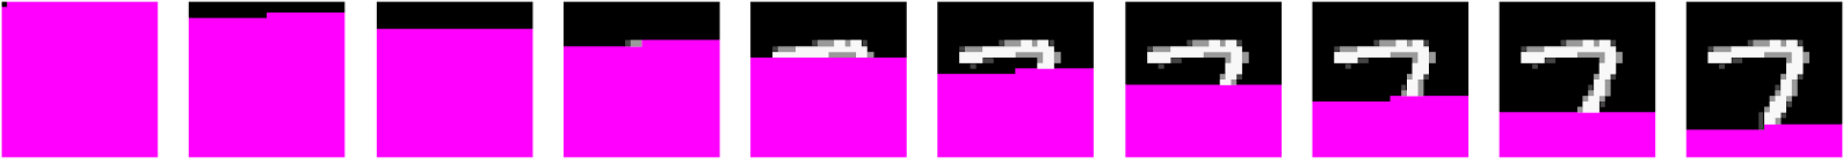
\includegraphics[width=0.7\linewidth]{figures/examples-sequential.png}
    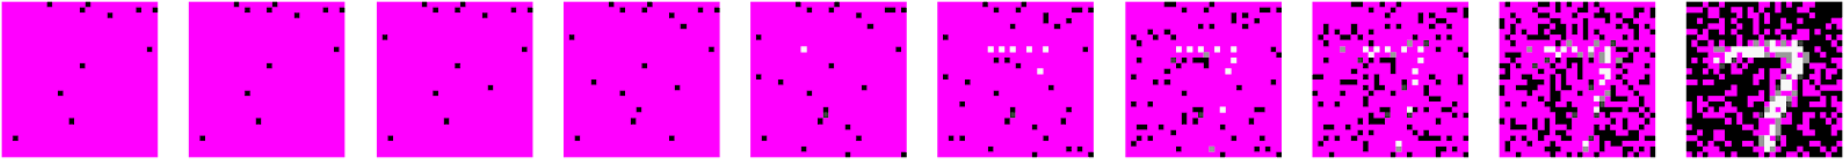
\includegraphics[width=0.7\linewidth]{figures/examples-random.png}
    \caption[Examples of the two MNIST training tasks]{Examples of the two tasks, showing input sequences with progressively more pixels filled in. (Pink means the pixel was not provided). Top: Pixels are presented in a contiguous forward-only order. Bottom: Pixels are presented in a non-contiguous, random order.}
    \label{fig:mnist-task-examples}
\end{figure}

In addition to the above encoding I experiment with three different pre-training task formats for the data. The first is forward-only auto-regressive pretraining as in the previous chapter (\Cref{fig:pretraining-causal}). The second is a ``Masked Sequence Modeling'' task, where I mask out a random subset of the pixels in the image, and the model is trained to predict the masked out pixels, and the final one is the ``Arbitrary-order auto-regressive pretraining`` variant I describe above in \Cref{sss:pretraining-triples}.

\subsection{Models}

\subsubsection{Architecture choices}

All model architectures shown here are transformer models, but they vary in the following ways:

\begin{enumerate}
    \item Absolute vs relative positional encodings
    \item Whether or not they include a ``query decoder''.
    \item If so, whether this decoder has a pooled input or not.
    \item Number of layers, embedding dimensionality etc.
\end{enumerate}



\section{Discussion}
\label{s:a-o-discussion}

As we can see in \Cref{fig:order-comparison}, the ``lowest-entropy-first'' ordering produces distinct images from the ``highest-entropy-first'' ordering. However, neither are as good as the ``random'' ordering.

Why do the ``lowest-entropy-first'' and ``highest-entropy-first'' orderings produce such different results? Why should they be different from the ``random'' ordering?

If the model has perfectly learned the true distribution of the data, then all orderings should produce the same results. However, the model is not perfect, and the ``random'' ordering is the only one that is not biased by the model's imperfections.

When we select a dynamic ordering based on the model's predictions, we are introducing a bias into the model's predictions. Let us examine this bias in more detail.

Let us imagine that the model outputs a gaussian =- more specifically it outputs estimates of the parameters $\mu$ and $\sigma$ of the true conditional distribution $p(y_i \mid x_i, y_{<i}, x_{<i})$. Then, also assume we can approximate the the fact that the model is imperfect by adding gaussian noise to the model's output, $\mu + \epsilon_\mu$ and $\sigma + \epsilon_\sigma$, where $\epsilon_\mu \sim \N(0, v_\mu)$ and $\epsilon_\sigma \sim \N(0, v_\sigma)$, for some small $v_\mu$ and $v_\sigma$. Let the model's output distribution be $q(i) = \N(y_i | x_i, y_{<i}, x_{<i}, \mu + \epsilon_\mu, \sigma + \epsilon_\sigma)$.

If we select the next position $i$ randomly, then when we sample $y_i \sim q(i)$, since the means of the error terms $\epsilon_\mu$ and $\epsilon_\sigma$ are both 0, the expected value of $y_i$ remains $\mu$.

However, when we select the next location $i$ to sample based on the entropy of $q(i)$, we select the location among many which has the highest (or lowest) variance $\sigma + \epsilon_\sigma$. On average, we will select a position with both high contribution from $\sigma$, \textbf{and} high contribution  from $\epsilon_\sigma$. Because of the high $\epsilon_\sigma$ term, this selection biases us towards sampling from distributions where the model is more uncertain than in the true distribution. We will therefore draw samples that are on average \textbf{less likely} in the true distribution. I.e. $\E[p(y_i \mid x_i, y_{<i}, x_{<i})] < \E[q(i)]$. To summarize, when we select an $i$ because the corresponding $q(i)$ has high entropy (variance), and then sample from this distribution, we will produce a pixel with a value that has $p(y) < q(y)$. The reverse is true for the ``lowest-entropy-first'' ordering. This is the bias that we are introducing into a \textit{single} prediction from the model.

I claim this same reasoning applies for the discrete case which I actually used in the experiment -- we can add an $\epsilon$ term to the logits, which when selecting for high entropy, pushes them towards the uniform distribution, and when selecting for low entropy, pushes them away. It so happens that on MNIST, this typically means the pixel will be brighter.

As we repeat this process, we will produce some pixels that are on average brighter than the true sequence. When the model is conditioned on these, it will generally infer that the remaining pixels should be brighter as well. This is why the ``highest-entropy-first'' ordering produces images that are as a whole brighter than the ``lowest-entropy-first'' ordering, and why both are shifted away from the ``random'' ordering.
